\subsection{Results}
\label{sec:dnds:results}

After the training and validation processes described in the previous Section, we have applied the fully trained CNN to the 14 years \fermi data. The result of our baseline analysis, which adopts the \verb|gll_iem_v07| galactic foreground and a latitude cut of $|b|<30^\circ$, is shown in Figure \ref{fig:prediction-fermi-12y}. The blue line is the reconstructed $\dnds$ and the error bands are the Bayesian errors obtained as described in Section \ref{sec:bayesian-error}. The blue points show the $\dnds$ of the resolved sources, obtained from the 4FGL-DR3 catalog. We can see that in the resolved limit, the CNN reconstructs a $\dnds$ fully compatible with the one derived from the catalog, but then extends it to the unresolved regime with a behaviour compatible with $\dnds \sim S^{-2}$ down to the smallest flux considered of $S = 5 \cdot 10^{-12}$ cm$^{-2}$ s$^{-1}$.
Below $S \sim  10^{-10}$ cm$^{-2}$ s$^{-1}$ the $\dnds$ exhibits a slight turn-up, although the feature has a very low statistical significance.

The result obtained here is also compatible with the one obtained in \cite{Cuoco-1pdf}, as shown in Figure \ref{fig:prediction-fermi-12y-vs-zechlin}. The difference between the two analyses, apart from the technique adopted to extract the $\dnds$, stands in the fact that here we update the data set to 14 years of \fermi data collection and to improved detector response functions, as compared to \cite{Cuoco-1pdf}. Another difference is that in \cite{Cuoco-1pdf} the  $\dnds$ was reconstructed with a broken power-law, while here we are allowing for a more flexible functional dependence (we are using 20 points in the flux interval shown in Figure \ref{fig:prediction-fermi-12y}). The result is nevertheless quite compatible with a power law behaviour with $\dnds \sim S^{-2}$ for mid-values of $S$, $\dnds \sim S^{-3}$ for $S > 10^{-8}$ cm$^{-2}$ s$^{-1}$ and a slight decrease in the power-law index for fluxes $S < 10^{-10}$ cm$^{-2}$ s$^{-1}$. 


In Figure \ref{fig:prediction-fermi-12y-bayesian} we show the measurement for the Fermi map employing the frequestist estimation of the error. It can be seen that the error is very similar to the Bayesian one, with some minimal difference at low fluxes. This provides confidence that the estimated error is robust. 






The CNN provides also the value $\fiso=4.90 \pm 0.43 \cdot 10^{-7}$ cm$^{-2}$ s$^{-1}$ sr$^{-1}$, 
which can be compared with the value $F'_\textrm{iso}=4.91 \pm 0.04 \cdot 10^{-7}$ cm$^{-2}$ s$^{-1}$ sr$^{-1}$ reported in Table \ref{tab:fore-parameters}.
We remind that $F'_\textrm{iso}$ is the sum of $\fiso$ and of the contribution of sources below the 4FGL catalog threshold. Indeed, if we  calculate the contribution of sources using our best fit $\dnds$ integrated in the range $[5 \cdot 10^{-12}, 1 \cdot 10^{-10}]$ cm$^{-2}$ s$^{-1}$, the upper limit being an approximate value for the catalog threshold, and we add $\fiso$  we obtain a value of {$(6.41 \pm 0.61)\cdot 10^{-7}$ cm$^{-2}$ s$^{-1}$} sr$^{-1}$.
This is in slight tension with $F'_\textrm{iso}$, although the two agree at the $\sim 2\sigma$ level.


In order to test the stability of the results, we repeated the analysis by using the same \verb|gll_iem_v07| galactic foreground but with two different latitude cuts: $|b|<40^\circ$ and $|b|<50^\circ$. The positive consequence of a higher latitude cut is a lower residual foreground contamination. However, the amount of available data is reduced. The CNN has been fully re-trained for both of these situations, and the ensuing results when applied to the \fermi data are shown in Figure \ref{fig:prediction-fermi-12y-b4050}. We notice that the results, both in terms of behaviour and uncertainty estimate, are fully compatible with the results of the baseline analysis. The $\dnds$ exhibits a slight decrease toward lower fluxes as compared to the baseline case, although the size of this effect is not statistically significant. The values of $\fiso$ are also fully compatible among them.

A second test of stability has been performed in order to check the impact of galactic foreground modeling. We have performed a new training of the CNN with the alternative template \verb|gll_iem_v05|, and with the $|b|<30^\circ$ latitude cut. The result is shown in Figure \ref{fig:prediction-fermi-12y-fg-v5}. The reconstructed $\dnds$ matches to a large degree the source-count distributions obtained with \verb|gll_iem_v07|. This reassures us that, even though the galactic foreground modeling introduces a degree of uncertainty, nevertheless the results of the CNN for $\dnds$ are remarkably stable.
The value of $\fiso$ is smaller in this case, equal to
$\fiso=1.82 \pm 0.15 \cdot 10^{-7}$ cm$^{-2}$ s$^{-1}$ sr$^{-1}$, 
which can be compared with the value $F'_\textrm{iso}=2.57 \pm 0.06 \cdot 10^{-7}$ cm$^{-2}$ s$^{-1}$ sr$^{-1}$ reported in table \ref{tab:fore-parameters}.
Adding to $\fiso$ the integral of the contribution of sources in the interval in the range $[5 \cdot 10^{-12}, 1 \cdot 10^{-10}]$ cm$^{-2}$ s$^{-1}$ using the obtained $\dnds$, we obtain a total flux of { $(2.92 \pm 0.54)\cdot 10^{-7}$ cm$^{-2}$ s$^{-1}$} sr$^{-1}$, which is in very good agreement with $F'_\textrm{iso}$. 






In Appendix \ref{furthertests}, we also discuss the results of further tests that we performed to cross-check the stability of the $\dnds$ derived in this section, and that confirm the  robustness of the result.  




\begin{figure}[t]
\centering
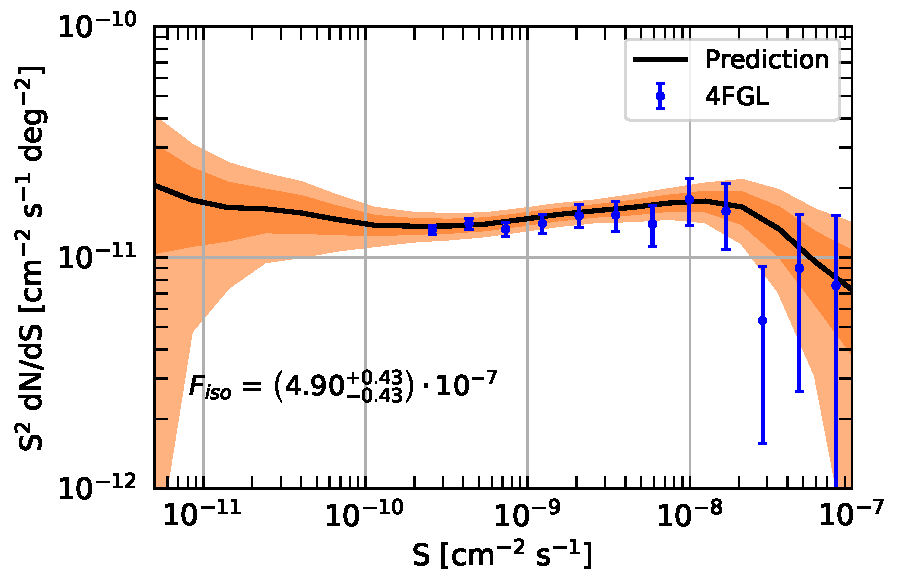
\includegraphics[width=0.9\textwidth]
{chapter_06/sections/paper_dnds/img/model_plots/model_42/baseline/fermi_prediction_hs.pdf}
\caption{Reconstructed $\dnds$ and $\fiso$  and their Bayesian errors, when the trained CNN is applied to the \fermi map. This is the main baseline result of the analysis.}
\label{fig:prediction-fermi-12y}
\end{figure}

\begin{figure}[t]
\centering
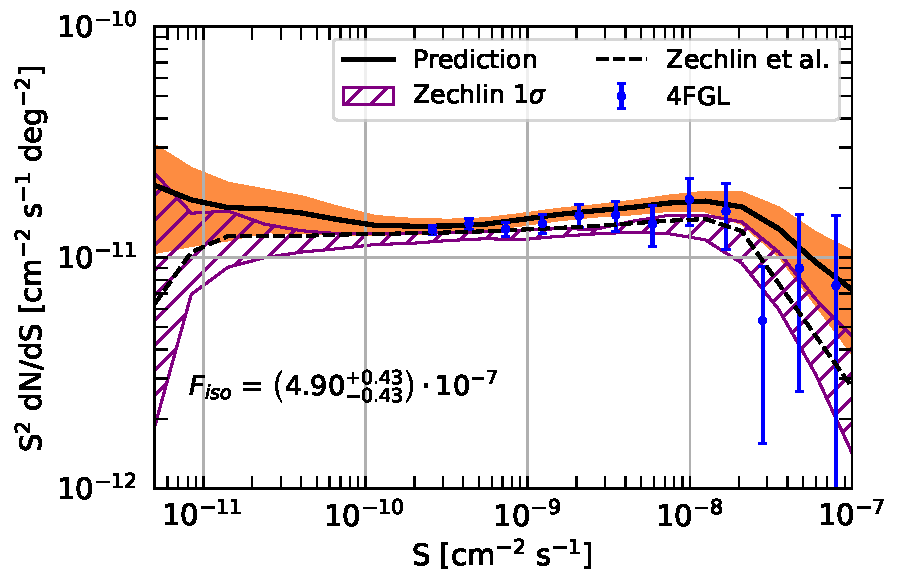
\includegraphics[width=0.9\textwidth]{chapter_06/sections/paper_dnds/img/model_plots/model_42/baseline/model_42_7e2_n64_flat_HL_comparison_with_paper.pdf}
\caption{Same as Figure \ref{fig:prediction-fermi-12y}, including a comparison with the result of Ref. \cite{Cuoco-1pdf}.}
\label{fig:prediction-fermi-12y-vs-zechlin}
\end{figure}

\begin{figure}[t]
\centering
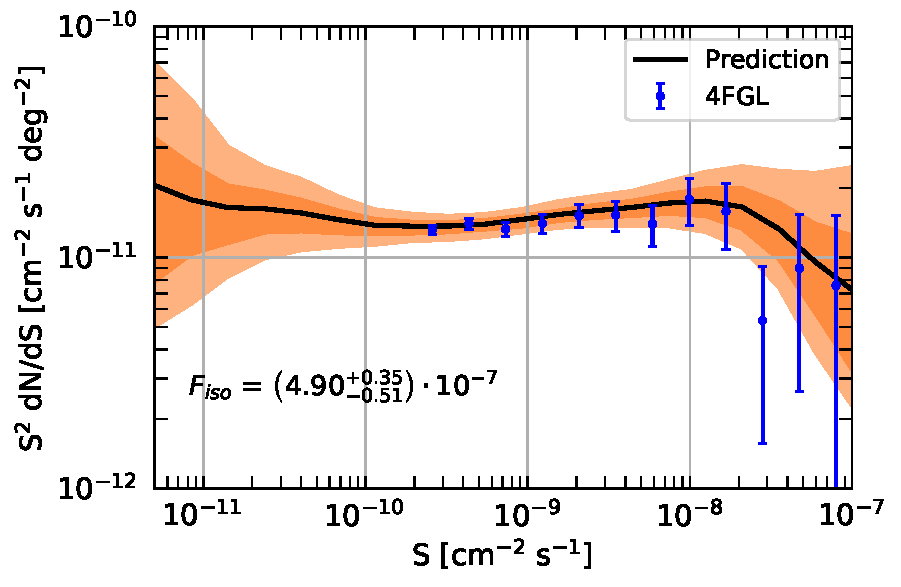
\includegraphics[width=0.9\textwidth]{chapter_06/sections/paper_dnds/img/model_plots/model_42/baseline/fermi_prediction_hist.pdf}
\caption{Same as in Figure \ref{fig:prediction-fermi-12y}, but with errors estimated through a frequentist approach.}
\label{fig:prediction-fermi-12y-bayesian}
\end{figure}

\begin{figure}[t]
\centering
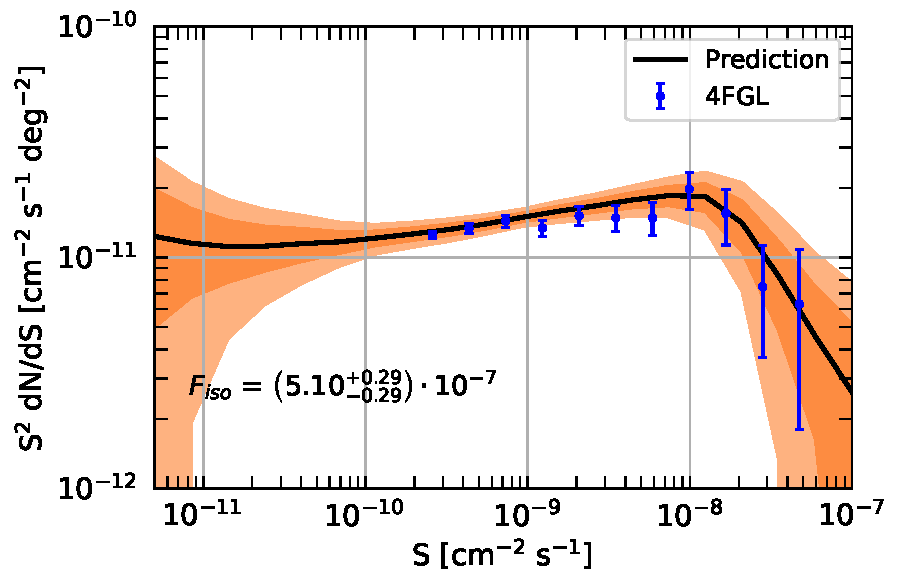
\includegraphics[width=0.9\textwidth]{chapter_06/sections/paper_dnds/img/model_plots/model_42/b40/fermi_prediction_hs.pdf}
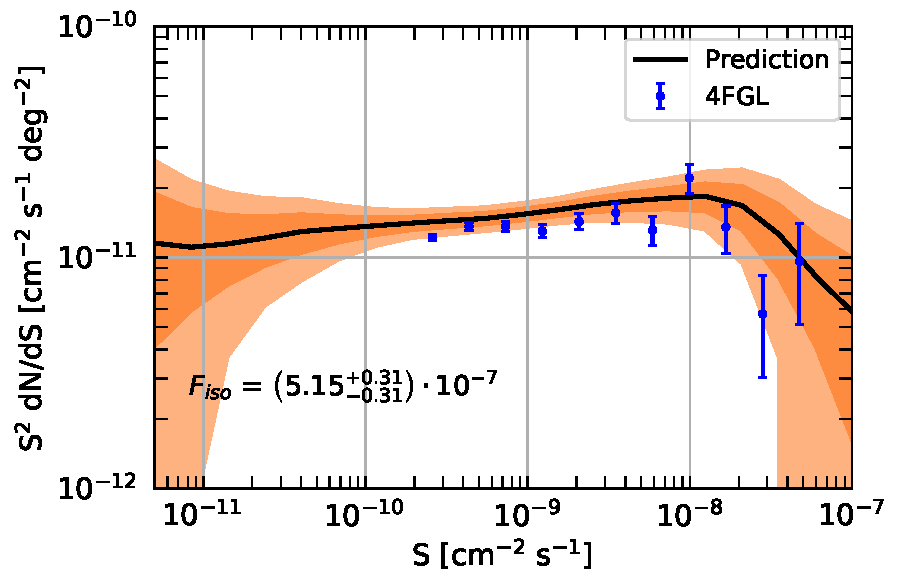
\includegraphics[width=0.9\textwidth]{chapter_06/sections/paper_dnds/img/model_plots/model_42/b50/fermi_prediction_hs.pdf}
\caption{Same as Figure \ref{fig:prediction-fermi-12y} but for a latitude cut of 40$^\circ$ and 50$^\circ$. The blue datapoints of the $\dnds$ of the 4FGL sources have been updated using only the source in the given region of interested. }
\label{fig:prediction-fermi-12y-b4050}
\end{figure}


\begin{figure}[t]
\centering
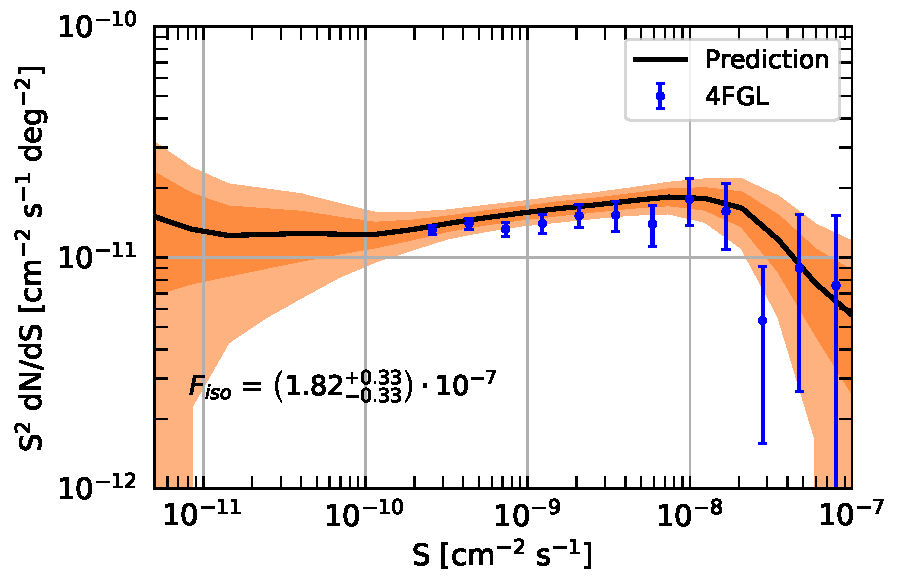
\includegraphics[width=0.9\textwidth]{chapter_06/sections/paper_dnds/img/model_plots/model_42/fg5/fermi_prediction_hs.pdf}
\caption{Same as Figure \ref{fig:prediction-fermi-12y} but using a CNN trained using the foreground model v05.}
\label{fig:prediction-fermi-12y-fg-v5}
\end{figure}



%---------------------------------

